\fchapter{Descripción de la práctica}

\fsection{Funcionamiento}

La práctica se ha realizado sobre la maqueta de horno Alecop MT-542, que dispone de una resistencia calefactora y de un ventilador, ambos con una entrada de mando externa. La temperatura del horno se mide con una sonda Pt100 que se conecta a la entrada de medida del controlador Omron E5EC. El controlador compara la temperatura medida con el punto de consigna (SP) fijado por el usuario y regula, mediante su salida de control 1, la resistencia calefactora del horno para mantener la temperatura en dicho valor.

\begin{figure}[H]
	\centering
	\includegraphics[height=9cm]{maqueta_mt542.jpg}
	\caption{Maqueta de horno Alecop MT-542}
\end{figure}

Se trata, por tanto, de un control automático en lazo cerrado. El controlador calcula el error ($e$) entre la consigna (SV) y la temperatura medida por la Pt100 (PV) y, a partir de él, el algoritmo PID determina la salida de control (MV) que se aplica a la resistencia calefactora. El calor aportado modifica la temperatura del horno, que vuelve a medirse y a realimentarse al controlador, cerrando el lazo:

\begin{figure}[H]
	\centering
	\resizebox{\linewidth}{!}{% Diagrama de bloques del lazo cerrado de control de temperatura
\shorthandoff{<>}% babel-spanish activa < y >, que TikZ necesita
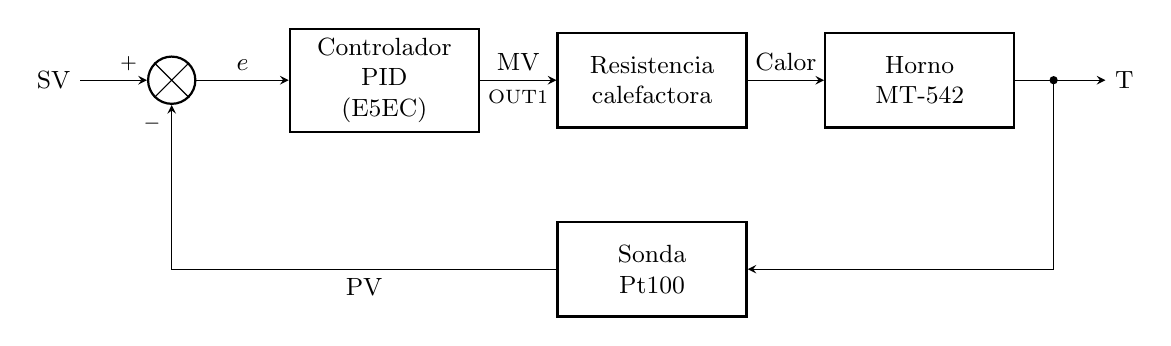
\begin{tikzpicture}[font=\small, >=stealth,
		bloque/.style={draw, thick, minimum height=1.2cm, minimum width=2.4cm, align=center},
		suma/.style={draw, thick, circle, minimum size=0.6cm, inner sep=0pt}]
	\node (sv) at (0,0) {SV};
	\node[suma] (s) at (1.5,0) {};
	\draw (s.north west) -- (s.south east) (s.north east) -- (s.south west);
	\node[bloque] (c) at (4.2,0) {Controlador\\PID\\(E5EC)};
	\node[bloque] (a) at (7.6,0) {Resistencia\\calefactora};
	\node[bloque] (p) at (11,0) {Horno\\MT-542};
	\node (t) at (13.6,0) {T};
	\node[bloque] (m) at (7.6,-2.4) {Sonda\\Pt100};

	\draw[->] (sv) -- (s.west) node[above left, font=\scriptsize]{$+$};
	\draw[->] (s.east) -- node[above]{$e$} (c.west);
	\draw[->] (c.east) -- node[above]{MV} node[below, font=\scriptsize]{OUT1} (a.west);
	\draw[->] (a.east) -- node[above]{Calor} (p.west);
	\draw[->] (p.east) -- (t.west);
	\draw[->] (12.7,0) |- (m.east);
	\draw[->] (m.west) -| node[pos=0.25, below]{PV} (s.south);
	\node[font=\scriptsize] at (1.25,-0.55) {$-$};
	\fill (12.7,0) circle (1.5pt);
\end{tikzpicture}
\shorthandon{<>}
}
	\caption{Esquema de lazo cerrado del control de temperatura}
\end{figure}

En esta práctica se ha trabajado con un punto de consigna de 55\,\textdegree C. Para señalizar el estado del proceso se han configurado cuatro alarmas, cada una asignada a una salida de relé del controlador que activa un elemento. Tres de ellas gobiernan los pilotos del módulo de señalización y la cuarta el ventilador de la maqueta:

\begin{itemize}
	\item \textbf{ALM1 -- Piloto amarillo:} se activa cuando la temperatura es inferior a 50\,\textdegree C, indicando que el horno todavía está frío.
	\item \textbf{ALM2 -- Piloto verde:} se activa cuando la temperatura está próxima a la consigna, desde 3\,\textdegree C por debajo hasta 1\,\textdegree C por encima del SV. Para una consigna de 55\,\textdegree C permanece encendido entre 52 y 56\,\textdegree C.
	\item \textbf{ALM3 -- Piloto rojo:} se activa cuando la temperatura supera los 60\,\textdegree C, indicando una temperatura elevada.
	\item \textbf{ALM4 -- Ventilador:} se activa cuando la temperatura supera en 2\,\textdegree C el punto de consigna (57\,\textdegree C para SV = 55\,\textdegree C), poniendo en marcha el ventilador para enfriar el horno.
\end{itemize}

\begin{table}[H]
	\centering
	\begin{tabularx}{\linewidth}{|C{2cm}|C{2.7cm}|Y|C{3cm}|}
		\hline
		\makecell{\textbf{Salida}} & \makecell{\textbf{Elemento}} & \makecell{\textbf{Condición de activación}} & \makecell{\textbf{Con SV = 55\,\textdegree C}} \\
		\hline
		ALM1 & Piloto amarillo & $PV < 50$\,\textdegree C & $< 50$\,\textdegree C \\
		\hline
		ALM2 & Piloto verde & $SV - 3 \leq PV \leq SV + 1$ & 52 -- 56\,\textdegree C \\
		\hline
		ALM3 & Piloto rojo & $PV > 60$\,\textdegree C & $> 60$\,\textdegree C \\
		\hline
		ALM4 & Ventilador & $PV \geq SV + 2$ & $\geq 57$\,\textdegree C \\
		\hline
	\end{tabularx}
	\caption{Resumen de las alarmas configuradas}
\end{table}

Las alarmas de los pilotos amarillo y rojo están referidas a temperaturas fijas (50 y 60\,\textdegree C), mientras que las del piloto verde y del ventilador están referidas al punto de consigna y se desplazan con él si este cambia.


\fsection{Montaje}

El montaje se ha realizado sobre el banco de trabajo del aula. Todas las conexiones se han hecho con cables de banana conectados directamente a las bornas del controlador, la maqueta, el módulo de señalización y las fuentes, sin necesidad de punteras.

Los elementos utilizados son los siguientes:

\begin{itemize}
	\item Controlador de temperatura Omron E5EC-QR4D5M-000, con alimentación de 24\,V AC/DC, salida de control 1 de tensión (12\,V DC para SSR), salida de control 2 de relé y cuatro salidas auxiliares de relé.
	\item Maqueta de horno Alecop MT-542, con resistencia calefactora y ventilador.
	\item Sonda Pt100 de tres hilos.
	\item Módulo de señalización con tres pilotos luminosos: amarillo, verde y rojo.
	\item Red de 230\,V AC, que alimenta las dos fuentes y la maqueta.
	\item Fuente de alimentación de 24\,V DC para el controlador.
	\item Fuente de alimentación regulable EP-603 (0 a 30\,V DC) para las cargas.
	\item Cables de banana para el conexionado.
\end{itemize}

\begin{figure}[H]
	\centering
	\includegraphics[height=10cm]{montaje_general.jpg}
	\caption{Montaje de la práctica en el banco de trabajo}
\end{figure}

\fsubsection{Alimentación}

Todo el conjunto se alimenta desde la red de 230\,V AC del banco, de la que toman tensión la maqueta del horno y las dos fuentes de alimentación. La fuente de las cargas se protege con los fusibles F3 y F4 en la fase y el neutro.

Se han utilizado dos fuentes de alimentación independientes. Una fuente de 24\,V DC alimenta el controlador E5EC a través de sus bornes 1 y 2, que no tienen polaridad al admitir tanto alterna como continua. La fuente regulable EP-603, ajustada a 12\,V DC, alimenta las cargas que conmutan los relés de alarma: los pilotos del módulo de señalización y el ventilador de la maqueta, cuya entrada externa admite como máximo 15\,V. De esta forma se separa la alimentación del equipo de control de la de las cargas.

\begin{figure}[H]
	\centering
	\begin{minipage}{0.48\linewidth}
		\centering
		\includegraphics[width=\linewidth]{fuente_24v.jpg}
		\caption{Fuente de 24\,V DC del controlador}
	\end{minipage}\hfill
	\begin{minipage}{0.48\linewidth}
		\centering
		\includegraphics[width=\linewidth]{fuente_ep603.jpg}
		\caption{Fuente regulable EP-603 para las cargas}
	\end{minipage}
\end{figure}

\fsubsection{Conexión de la sonda Pt100}

La sonda Pt100 es de tres hilos y se conecta a la entrada de sensor del controlador, que en el E5EC corresponde a los bornes 22, 23 y 24. El extremo A de la resistencia de la Pt100 va al borne 22 y los dos hilos del extremo B van a los bornes 23 y 24, de modo que la resistencia de medida queda entre los bornes 22 y 23. El tercer hilo, conectado al borne 24, permite al controlador compensar la resistencia de los cables, de modo que la longitud del cableado no falsea la medida de temperatura.

\begin{table}[H]
	\centering
	\begin{tabularx}{0.6\linewidth}{|C{2cm}|C{2cm}|Y|}
		\hline
		\makecell{\textbf{Borne}} & \makecell{\textbf{Terminal Pt}} & \makecell{\textbf{Conexión}} \\
		\hline
		22 & A & Extremo A de la Pt100 \\
		\hline
		23 & B & Extremo B de la Pt100 \\
		\hline
		24 & B & Hilo de compensación (extremo B) \\
		\hline
	\end{tabularx}
	\caption{Conexión de la Pt100 a la entrada del E5EC}
\end{table}

\begin{figure}[H]
	\centering
	\includegraphics[width=0.85\linewidth]{etiqueta_bornes_e5ec.jpg}
	\caption{Etiqueta de bornes del E5EC y conexión de la sonda Pt100 en los bornes 22, 23 y 24}
\end{figure}

\fsubsection{Salida de control}

La salida de control 1 del E5EC es una salida de tensión de 12\,V DC, disponible entre los bornes 3 ($+$) y 4 ($-$). Se ha conectado a la entrada externa de mando de la resistencia calefactora de la maqueta, con el conmutador de la resistencia en posición \textit{ext}, y el borne 4 al 0\,V de la maqueta. La potencia de la resistencia la proporciona la propia maqueta; el controlador solo le envía la orden de conexión, activando y desactivando la salida en función del cálculo del PID.

\fsubsection{Salidas de alarma}

Las cuatro alarmas se han asignado a las salidas auxiliares de relé del controlador: ALM1 al piloto amarillo, ALM2 al piloto verde, ALM3 al piloto rojo y ALM4 al ventilador. En el E5EC las salidas auxiliares comparten borne común por parejas: el borne 11 es común de las salidas 1 y 2, y el borne 8 es común de las salidas 3 y 4.

El positivo de 12\,V DC de la fuente EP-603 se ha puenteado a los dos bornes comunes (8 y 11). Cada borne de salida de alarma se lleva a su elemento correspondiente y el otro extremo de todos los elementos se conecta al negativo (0\,V) de la misma fuente. En el caso del ventilador, su conmutador se coloca en posición \textit{ext} para que sea gobernado desde la entrada externa. Así, cuando una alarma se activa, su relé cierra el contacto entre el común y la salida y el elemento queda alimentado.

\begin{table}[H]
	\centering
	\begin{tabularx}{0.8\linewidth}{|C{2cm}|C{2.5cm}|Y|}
		\hline
		\makecell{\textbf{Salida}} & \makecell{\textbf{Bornes}} & \makecell{\textbf{Elemento}} \\
		\hline
		ALM1 & 11 (común) -- 12 & Piloto amarillo \\
		\hline
		ALM2 & 11 (común) -- 10 & Piloto verde \\
		\hline
		ALM3 & 8 (común) -- 9 & Piloto rojo \\
		\hline
		ALM4 & 8 (común) -- 7 & Ventilador \\
		\hline
	\end{tabularx}
	\caption{Conexionado de las salidas de alarma del E5EC}
\end{table}

\begin{figure}[H]
	\centering
	\begin{minipage}{0.48\linewidth}
		\centering
		\includegraphics[height=8cm]{bornes_e5ec.jpg}
		\caption{Cableado de los bornes del E5EC}
	\end{minipage}\hfill
	\begin{minipage}{0.48\linewidth}
		\centering
		\includegraphics[height=8cm]{modulo_senalizacion.jpg}
		\caption{Módulo de señalización}
	\end{minipage}
\end{figure}


\fsection{Esquemas}

En la figura siguiente se muestra el esquema eléctrico completo de la instalación: la red de 230\,V AC con las dos fuentes y sus protecciones, la alimentación del controlador, la conexión de la sonda Pt100 a tres hilos, la salida de control 1 hacia la entrada externa de la resistencia de la maqueta y las cuatro salidas auxiliares de alarma, con sus comunes puenteados al positivo de la fuente de cargas.

\begin{figure}[H]
	\centering
	\rotatebox{90}{\begin{minipage}{0.9\textheight}
		\centering
		\resizebox{\linewidth}{!}{% Esquema eléctrico de la instalación (circuitikz)
\begin{circuitikz}[european, scale=0.72, transform shape, font=\small]
	% ---------------- Red 230 V AC ----------------
	\draw[thick] (-9,18) node[left]{L} -- (18,18);
	\draw[thick] (-9,17.3) node[left]{N} -- (18,17.3);
	\node[anchor=west, font=\scriptsize] at (-9,18.35) {230\,V AC};

	% ---------------- Controlador E5EC ----------------
	\draw[thick] (0,0.3) rectangle (4,13.5);
	\node[align=center] at (2,14.1) {\textbf{Omron E5EC-QR4D5M-000}};
	% Bornes lado izquierdo
	\foreach \y/\b in {12/1, 10.5/2, 8.5/3, 7/4} {
		\draw (0,\y) node[ocirc]{} node[right, font=\scriptsize]{\b};
	}
	% Bornes lado derecho
	\foreach \y/\b/\f in {12/11/COM, 11/8/COM, 9.5/12/AUX1, 8.5/10/AUX2, 7.5/9/AUX3, 6.5/7/AUX4} {
		\draw (4,\y) node[ocirc]{} node[left, font=\scriptsize]{\f\ \b};
	}
	\foreach \y/\b in {3/22, 2/23, 1/24} {
		\draw (4,\y) node[ocirc]{} node[left, font=\scriptsize]{\b};
	}
	\node[align=left, anchor=west, font=\scriptsize] at (0.6,11.25) {24\,V AC/DC};
	\node[align=left, anchor=west, font=\scriptsize] at (0.6,7.75) {OUT1\\12\,V DC};
	\node[align=right, anchor=east, font=\scriptsize] at (3.2,2) {Entrada\\Pt100};

	% ---------------- Fuente 1: alimentación del controlador ----------------
	\draw[thick] (-4,13.8) rectangle (-2,15.6);
	\draw (-4,13.8) -- (-2,15.6);
	\node[font=\scriptsize] at (-3.45,15.2) {AC};
	\node[font=\scriptsize] at (-2.55,14.2) {DC};
	\node[align=right, anchor=east, font=\scriptsize] at (-4.1,14.7) {Fuente 1\\24\,V DC};
	\draw (-3.5,15.6) -- (-3.5,18) node[circ]{};
	\draw (-2.5,15.6) -- (-2.5,17.3) node[circ]{};
	\draw (-2.5,13.8) -- (-2.5,12) -- (0,12) node[above left, font=\scriptsize]{$+$};
	\draw (-3.5,13.8) -- (-3.5,10.5) -- (0,10.5) node[above left, font=\scriptsize]{$-$};

	% ---------------- Maqueta: resistencia gobernada por OUT1 ----------------
	\draw (0,8.5) node[above left, font=\scriptsize]{$+$} -- (-4.3,8.5);
	\draw (0,7) node[below left, font=\scriptsize]{$-$} -- (-4.3,7);
	\draw[thick] (-8.3,6.3) rectangle (-4.3,9.2);
	\node[align=center, font=\scriptsize] at (-6.3,7.75) {Maqueta MT-542\\Resistencia calefactora\\entrada ext. (0--10\,V)};
	\draw (-4.3,8.5) node[ocirc]{} node[left, font=\scriptsize]{ext};
	\draw (-4.3,7) node[ocirc]{} node[left, font=\scriptsize]{0\,V};
	\draw (-7,9.2) node[ocirc]{} -- (-7,18) node[circ]{};
	\draw (-5.6,9.2) node[ocirc]{} -- (-5.6,17.3) node[circ]{};

	% ---------------- Sonda Pt100 a 3 hilos ----------------
	\draw (4,3) node[above right, font=\scriptsize]{A} -- (6.3,3)
		to[R, l^=Pt100] (6.3,-0.3) -- (5.5,-0.3) node[circ]{};
	\draw (5.5,-0.3) -- (5.5,2) -- (4,2) node[above right, font=\scriptsize]{B};
	\draw (5.5,-0.3) -- (5,-0.3) -- (5,1) -- (4,1) node[above right, font=\scriptsize]{B};

	% ---------------- Fuente 2 (EP-603): alimentación de las cargas ----------------
	\draw (15.5,18) node[circ]{} to[fuse, l_=F3] (15.5,15.6);
	\draw (16.5,17.3) node[circ]{} to[fuse, l^=F4] (16.5,15.6);
	\draw[thick] (15,13.8) rectangle (17,15.6);
	\draw (15,13.8) -- (17,15.6);
	\node[font=\scriptsize] at (15.55,15.2) {AC};
	\node[font=\scriptsize] at (16.45,14.2) {DC};
	\node[align=left, anchor=west, font=\scriptsize] at (17.1,14.7) {Fuente 2\\EP-603\\12\,V DC};

	% ---------------- Salidas de alarma ----------------
	% Puente de los comunes al +12 V
	\draw (4,12) -- (5,12) node[circ]{};
	\draw (4,11) -- (5,11) -- (5,13) -- (15.5,13) node[above right, font=\scriptsize]{$+$} -- (15.5,13.8);
	% Cargas
	\draw (4,9.5) -- (14,9.5) to[lamp] (14,3.8);
	\node[align=left, anchor=west, font=\scriptsize] at (14.5,6.6) {P1\\Piloto\\amarillo\\(ALM1)};
	\draw (4,8.5) -- (12,8.5) to[lamp] (12,3.8);
	\node[align=left, anchor=west, font=\scriptsize] at (12.5,6.1) {P2\\Piloto\\verde\\(ALM2)};
	\draw (4,7.5) -- (9.5,7.5) -- (9.5,6.4);
	\draw (9.5,5.8) circle (0.6) node{M};
	\draw (9.5,5.2) -- (9.5,3.8);
	\node[align=left, anchor=west, font=\scriptsize] at (10.15,5.8) {Ventilador\\(ALM4)};
	\draw (4,6.5) -- (7,6.5) to[lamp] (7,3.8);
	\node[align=left, anchor=west, font=\scriptsize] at (7.5,5.1) {P3\\Piloto\\rojo\\(ALM3)};
	% Retorno a 0 V
	\draw (7,3.8) node[circ]{} -- (9.5,3.8) node[circ]{} -- (12,3.8) node[circ]{} -- (14,3.8) node[circ]{} -- (16.5,3.8) -- (16.5,13.8);
	\node[font=\scriptsize, anchor=west] at (16.6,12.8) {0\,V};
\end{circuitikz}
}
		\captionof{figure}{Esquema eléctrico de la instalación}
	\end{minipage}}
\end{figure}
